%%%%%%%%%%%%%%%%%%%%%%%%%%%%%%%%%%%%%%%%%%%%%%%%%%%%%%%%%%%%%%%%%%%%%%%%%%%
%
% Template for a LaTex article in English.
%
%%%%%%%%%%%%%%%%%%%%%%%%%%%%%%%%%%%%%%%%%%%%%%%%%%%%%%%%%%%%%%%%%%%%%%%%%%%

\documentclass{article}

% AMS packages:
\usepackage{amsmath, amsthm, amsfonts}
\usepackage[margin=2cm]{geometry}% by courtesy of Micro
\usepackage{pgfplots}
\usepackage{tikz}
\usepackage{tcolorbox}
\usetikzlibrary{arrows,shapes.geometric,fit,matrix}
\usetikzlibrary{backgrounds,calc,chains,decorations,positioning}

\tcbset{
    nobeforeafter,
    %colbacktitle=blue!20,
    %colback=yellow!30,
    %coltitle=black,
    %coltext=black,
    %fontupper=\sffamily\bfseries\LARGE,
    %width=.5\linewidth,
}

% Theorems
%-----------------------------------------------------------------
\newtheorem{thm}{Theorem}[section]
\newtheorem{cor}[thm]{Corollary}
\newtheorem{lem}[thm]{Lemma}
\newtheorem{prop}[thm]{Proposition}
\theoremstyle{definition}
\newtheorem{defn}[thm]{Definition}
\theoremstyle{remark}
\newtheorem{rem}[thm]{Remark}

% Shortcuts.
% One can define new commands to shorten frequently used
% constructions. As an example, this defines the R and Z used
% for the real and integer numbers.
%-----------------------------------------------------------------
\def\RR{\mathbb{R}}
\def\ZZ{\mathbb{Z}}

% Similarly, one can define commands that take arguments. In this
% example we define a command for the absolute value.
% -----------------------------------------------------------------
\newcommand{\abs}[1]{\left\vert#1\right\vert}

% Operators
% New operators must defined as such to have them typeset
% correctly. As an example we define the Jacobian:
% -----------------------------------------------------------------
\DeclareMathOperator{\Jac}{Jac}

%-----------------------------------------------------------------
\title{Ternary Parallel \LaTeX\ Plot $02$}
\author{Rajdeep Chatterjee\\
  \small School of Computer Engineering\\
  \small KIIT Deemed to be University\\
  \small Bhubaneswar 751024, India
}

\begin{document}
\maketitle

\tikzset{near start abs/.style={xshift=1cm}}

\begin{figure}[!ht]
 \centering
 \scalebox{0.8}{
 \resizebox{\columnwidth}{!}{%
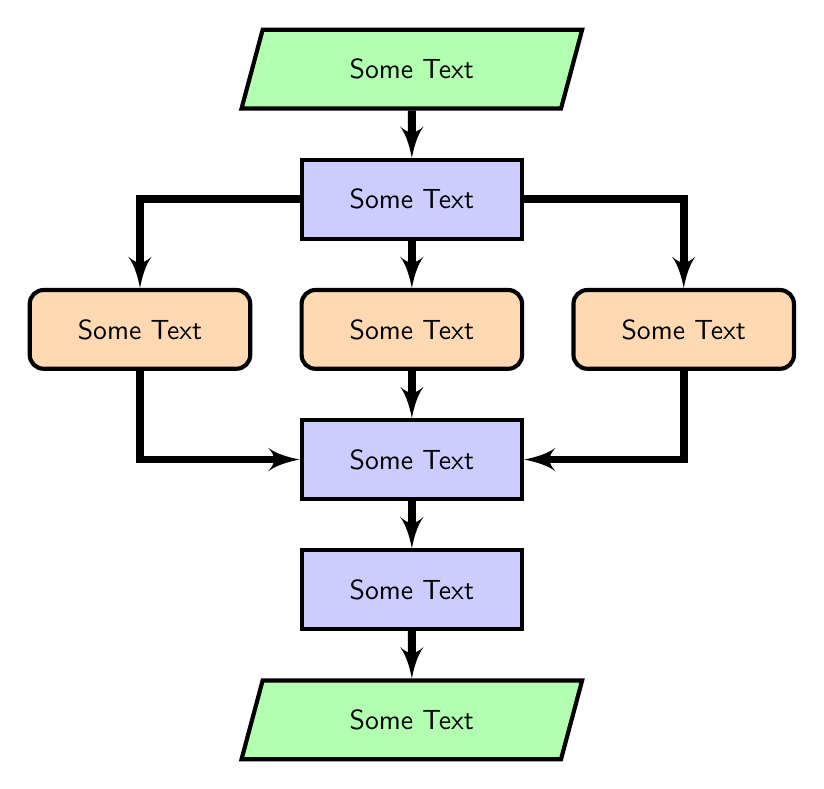
\begin{tikzpicture}[node distance=6mm, >=latex',
block/.style = {draw, rectangle, minimum height=10mm, minimum width=28mm,align=center, fill=blue!20, font=\sffamily},
rblock/.style = {draw, rectangle, rounded corners=0.5em, minimum height=10mm, minimum width=28mm,align=center, fill=orange!30, font=\sffamily},
tblock/.style = {draw, trapezium, minimum width=10mm, minimum height=10mm,
                 trapezium left angle=75, trapezium right angle=105, align=center, fill=green!30, font=\sffamily},
                    ]
    %\node [rblock,line width=1.5pt]                       (start){Start};
    \node [tblock, line width=1.5pt]       (input){Some Text};
    \node [block, below=of input,line width=1.5pt]       (preprocess){Some Text};
    \node [rblock, below=of preprocess,line width=1.5pt]      (detect2){Some Text};
    \node [rblock, left=of detect2,line width=1.5pt]      (detect1){Some Text};
    \node [rblock, right=of detect2,line width=1.5pt]      (detect3){Some Text};
    \node [block, below=of detect2,line width=1.5pt]         (mask){Some Text};
    \node [block, below=of mask,line width=1.5pt]    (closing){Some Text};
    \node [tblock, below=of closing,line width=1.5pt]  (result){Some Text};
    \path[draw=black,solid,line width=1mm,fill=black,->]
                   %(start)      edge (input)
                   (input)    edge (preprocess)
                   (preprocess)   edge (detect2)
                   (detect2)  edge (mask)
                   (mask)   edge (closing)
                   (closing)  edge (result)
                    ;
    \draw[solid,line width=1mm,->] (preprocess)   -| (detect1);
    \draw[solid,line width=1mm,->] (preprocess)   -| (detect3);
    \draw[solid,line width=1mm,->] (detect1)   |- (mask);
    \draw[solid,line width=1mm,->] (detect3)   |- (mask);
\end{tikzpicture}}
} \caption{Place your caption here}
\label{fig2}
\end{figure}

\end{document}
